\documentclass[10pt,a4paper,pdftex]{book}

\input{En_tete/packages.tex}
\input{En_tete/informatique.tex}
\input{En_tete/mise_en_page.tex}
\input{En_tete/raccourcis.tex}



%\usepackage[nosolutionfiles]{answers} %% A selectionner pour avoir le corrigé sous la question
\usepackage{answers} %% A selectionner pour avoir le corrigé à part

%%%%%%%%%%%%%%%%%%%%%%%%%%%%%%%%%%%%%%%%%%%%%%%%%%%%%%%%%%%%%%%%%%%%%%
%%%%%%%%%%% Définition des réponses aux questions %%%%%%%%%%%%%%%%%%%%
%%%%%%%%%%%%%% = utilisation du package answers %%%%%%%%%%%%%%%%%%%%%%
%%%%%%%%%%%%%%%%%%%%%%%%%%%%%%%%%%%%%%%%%%%%%%%%%%%%%%%%%%%%%%%%%%%%%%
%%% Les réponses aux questions
\Newassociation{reponse}{Rep}{Corrige_chp9}
%Le nom de l'environnement est "reponse", le compteur "Rep", et le fichier qui récupère "Corrige"
\renewcommand{\Replabel}[1]{{\bigskip \noindent \hypertarget{ex:#1}{}
\hyperlink{sol:#1}{\tcbox[enhanced,colback=white,drop shadow northwest,size=fbox,on line]
{\textbf{Solution #1}}}
 \hspace{0.2cm}}}
%% Pour mettre des commentaires envoyés dans le corrigé (n'apparait pas dans le corrigé dessous)
%   \begin{Filesave}{Corrige}}
%   \end{Filesave}}
%%%%%%%%%%%%%%%%%%%%%%%%%%%%%%%%%%%%%%%%%%%%%%%%%%%%%%%%%%%%%%%%%%%%%
%%%%%%%%%%%%%%%% Fin structuration des réponses  %%%%%%%%%%%%%%%%%%%%
%%%%%%%%%%%%%%%%%%%%%%%%%%%%%%%%%%%%%%%%%%%%%%%%%%%%%%%%%%%%%%%%%%%%%

\begin{document}

%%%%%%%%%%%%%%%%%%%%%%%%%%%%%%%%%%%%%%%%%%%%%%%%%%%%%%%%%%%%%%%%%%%%%
%%%%%%%%%%%%%%%%%%%%%%%%%% Mini TOC %%%%%%%%%%%%%%%%%%%%%%%%%%%%%%%%%
%%%%%%%%%%%%%%%%%%%%%%%%%%%%%%%%%%%%%%%%%%%%%%%%%%%%%%%%%%%%%%%%%%%%%
\dominitoc
\mtcsettitlefont{minitoc}{\large\scshape}
\renewcommand{\mtctitle}{Table des matières}

%%%%%%%%%%%%%%%%%%%%%%%%%%%%%%%%%%%%%%%%%%%%%%%%%%%%%%%%%%%%%%%%%%%%%
%%%%%%%%%%%%%%%%%%%%%%% Début du cours %%%%%%%%%%%%%%%%%%%%%%%%%%%%%%
%%%%%%%%%%%%%%%%%%%%%%%%%%%%%%%%%%%%%%%%%%%%%%%%%%%%%%%%%%%%%%%%%%%%%
\renewcommand{\labelitemi}{$\star$}
\pagestyle{perso}

\setcounter{chapter}{9}
\chapter{Les Images}
\minitoc

\Opensolutionfile{Corrige_chp9}
\begin{Filesave}{Corrige_chp9}
\newpage
\section{Solutions des exercices}
\end{Filesave}

\newpage
\section{Représentation informatique d'une image} 


Il existe deux grands types de représentations pour les images.

\medskip
La \defi{représentation vectorielle}, pour les images qu'on peut représenter à partir d'un nombre fini de figures  géométriques élémentaires. Le fichier image contient alors une suite d'instructions de tracé exprimées dans un langage de programmation.

\medskip
La \defi{représentation bitmap}, avec laquelle nous travaillerons, où l'image est quadrillée selon une matrice de $largeur \times hauteur$ cases, appelées \defi{pixels} (\textit{picture element}). Chaque pixel code la couleur d'un petit carré de l'image à l'aide de 1, 3 ou 4 valeurs suivant le type d'image. 

\smallskip
\begin{itemize}
	\item Pour une image en niveaux de gris, la couleur de chaque pixel est codée sur un octet (8 bits), ce qui permet d'obtenir $2^8 = 256$ valeurs possibles (de 0 à 255). Par exemple, la valeur 0 code la couleur noir et la valeur 255 code le blanc.
	\item Pour une image en couleur, le codage le plus utilisé est le codage RGB (RedGreenBlue). Ici, la couleur d'un pixel est codée
sur 3 octets ($3\times 8$ bits) par un triplet de trois entiers compris entre 0 et 255 : le premier entier code la quantité de rouge, le deuxième la quantité de vert et le troisième la quantité de bleu. La couleur du pixel est obtenue par synthèse additive de ces trois couleurs. Par exemple, le triplet $(0, 0, 0)$ correspond au noir, $(200, 200, 200)$ à un gris clair, $(255, 0, 0)$ à un rouge éclatant, $(255, 255, 0)$ à un jaune vif (rouge + vert), $(255, 127, 0)$ à du orange\dots\ Finalement une image en couleur est la superposition de trois images monochromes (cf exercice \ref{monochrome})
	\item Pour une image en couleur, on utilise également 
\end{itemize}

\medskip
Il existe d'autres façons de représenter des images en couleurs, notamment le codage RGBA (RedGreenBlueAlpha). Dans ce cas, la couleur d'un pixel est codée sur 4 octets par quatre entiers compris entre 0 et 255 : les trois premiers entiers codent la quantité de rouge, de vert et de bleu, le quatrième entier code la transparence de la couleur. Ou encore \og \textsc{cymk}\fg{} très utile pour l'impression, mais nous ne travaillerons lors de ce \textsc{tp} qu'avec les deux premières évoquées.

\medskip

Les fichiers images de type bitmap sont adaptés à la représentation de figures aux contours irréguliers, en photographie par exemple. Le format \texttt{bmp} permet une simple description pixel par pixel, le poids de l'image est alors $Largeur\times Hauteur\times 3\ octets$. Les fichiers images peuvent donc être de grande taille, pour cela ils sont souvent compressés avec ou sans perte d'information.
Les formats \texttt{png} et \texttt{jpg} sont des exemples de formats d'images bitmap compressés. Pour le premier la compression est réversible (c'est-à-dire sans perte d'information), pour le second c'est avec perte d'information, mais le taux de compression est plus important.

\ex d'un système de compression : $(1,1,0,0,0,1,1,1,1,0,1,1,1,0,\ldots)\longrightarrow (1,2,3,4,1,3,\ldots)$.


\section{Traitement d'images en Python}

Nous aurons trois niveaux d'abstraction pour traiter nos images. Le fichier physique sur le disque (\texttt{png}, \texttt{jpg} par exemple). L'\og objet Python\fg{} intermédiaire (on ne s'en occupera pas vraiment). Et enfin la matrice des pixels sur laquelle on opèrera.  

\medskip
Pour traiter l'\og objet Python intermédiaire\fg{} nous utiliserons le module \texttt{Image} de la bibliothèque \texttt{PIL} (Python Imaging Library). \verb!PIL!  ne fait pas partie de la bibliothèque standard de Python : il s'agit d'une bibliothèque supplémentaire (libre) qu'il faut installer. Pour se faire il faut avoir une connexion internet et dans l'interpréteur Python il suffit de taper une des deux lignes suivantes :
\begin{lstlisting}[style=compil]
>>> pip install Pillow
>>> conda install Pillow
\end{lstlisting}
l'installation se fera automatiquement. La documentation  est  disponible à partir de la  page web \url{http://effbot.org/imagingbook/pil-index.htm}.

\medskip
Pour travailler avec les matrices nous utiliserons la bibliothèque \texttt{numpy}. C'est un outils très puissant déjà installé avec Pyzo et dont vous aurez l'occasion de vous servir notamment en algèbre linéaire l'an prochain.

\Rq On peut faire du traitement d'image avec d'autres modules de python \texttt{matplotlib.pyplot}, \texttt{imageio} par exemple.

\medskip
Avant de commencer ce \textsc{tp}, prenez soin de créer un répertoire dans lequel vous allez travailler. Vous y copierez depuis le dossier de partage : le fichier \texttt{.py} dans lequel une partie des codes est déjà tapé, les images que nous utiliserons.

Pensez aussi que vous allez travailler avec des fichiers, et comme dans le \textsc{tp} précédent lors de la première exécution vous prendrez soin de faire \texttt{Exécuter / Démarrer le script}.

\medskip Dans ce qui suit nous allons décrire les principales commandes dont nous aurons besoin pour la suite.

\begin{lstlisting}
from PIL import Image
import numpy as np

im = Image.open("nom_fichier.extension") # "objet python" intermédiaire.
im.show()	# affiche l'image dans une fenêtre graphique
pixels = np.array(im) # matrice des pixels
hauteur, largeur = pixels.shape[:2] # dimensions de la matrice
\end{lstlisting}

\Rqs 
\begin{itemize}
\item \texttt{pixels} est un objet de type \texttt{array} (tableau). Chaque élément qui le compose est un entier (non signé) compris entre 0 et 255.
\item Si on travaille avec une image en couleur \texttt{pixels.shape} renverra un triplet (hauteur, largeur, 3), si on travaille avec une image en niveau de gris \texttt{pixels.shape} renvoie directement le couple (hauteur, largeur). En imposant de ne renvoyer que les deux première composantes avec la commande \texttt{pixels.shape[:2]} on n'a pas à se soucier si on travaille en niveau de gris ou en couleur.
\end{itemize}



\bigskip
Un des buts de ce \textsc{tp} est de faire du traitement d'image, c'est à dire modifier la luminosité, le contraste, appliquer des filtres \ldots\ On va donc être amené à modifier la valeur des pixels, voici donc comment accéder à ces valeurs et comment les modifier. (on supposera que la matrice des pixels se nomme \texttt{pixels})

\begin{lstlisting}
couleur=pixels[i,j]
# On récupère la couleur du pixel situé sur la i-ième ligne et la j-ième colonne.
\end{lstlisting}
Si l'image est en couleur on obtiendra un triplet (en fait un \texttt{array} avec 3 éléments) correspondant à la quantité de rouge de vert et de bleu. Si l'image est en niveau de gris on aura un seul entier.

\medskip
Pour ne pas perdre les données de la matrice initiale, on ne travaillera jamais sur celle-là, on va en créer une nouvelle ayant les mêmes caractéristiques (hauteur, largeur, nombre de couleurs) que la première.
\begin{lstlisting}
pixels_res = np.zeros_like(pixels) # Une matrice qu'avec des zéros
pixels_res = np.copy(pixels) # Une copie en profondeur
\end{lstlisting}

Ensuite pour modifier les pixels on peut par exemple procéder ainsi
\begin{lstlisting}
pixels[i,j]=[255,255,255]
# Le pixel de coordonnées (i,j) est colorié en blanc (image en couleur).
pixels[i,j]=255
# Le pixel de coordonnées (i,j) est colorié en blanc (image en niveau de gris).
\end{lstlisting}

Une fois toutes les manipulations faites il faut transformer la matrice en une image et l'enregistrer sur le disque. 
\begin{lstlisting}
img_res = Image.fromarray(pixels_res)
img_res.save("nouveau_fichier.extension")
# enregistre la nouvelle image dans le fichier nouveau_fichier.extension
\end{lstlisting}


\ex Voici l'exemple d'une fonction qui permet de créer l'image miroir d'une autre image (pour cela, il \og suffit\fg{} d'inverser l'ordre des colonnes de la matrice des pixels de l'image de départ) :
\begin{lstlisting}
def miroir(fichier):
    """prend en entrée un fichier image et retourne l'image de l'image
     obtenue par une réflexion par rapport à l'axe vertical droit
    """
    im=Image.open(fichier)
    pixels = np.array(im)
    hauteur, largeur = pixels.shape[:2]
    pixels_res = np.zeros_like(pixels)
    for i in range(hauteur):
        for j in range(largeur):
            pixels_res[i, j,:] = pixels[i, largeur - 1 -  j,:]
    img_res = Image.fromarray(pixels_res)
    img_res.save("miroir"+fichier)
    img_res.show()
\end{lstlisting}

Après avoir exécuter la fonction, on l'appelle de la manière suivante.
\begin{lstlisting}[style=compil]
>>> miroir("valleluna.jpg")
\end{lstlisting}

On obtient alors quelque chose qui ressemble à ce qui suit.
\begin{center}
\begin{tabular}{cp{2cm}c}
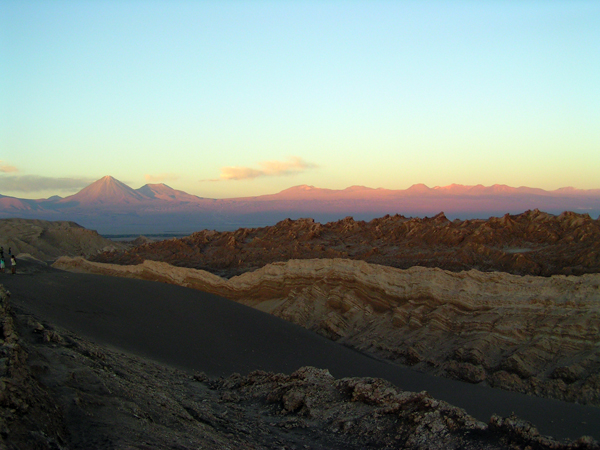
\includegraphics[scale=0.3]{Images/valleluna.jpg}
& &
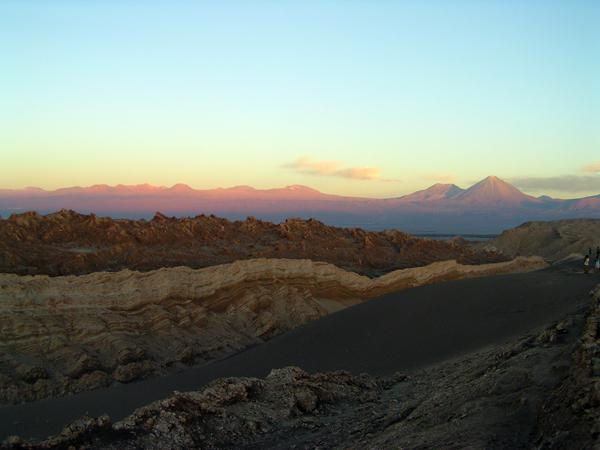
\includegraphics[scale=0.3]{Images/miroir_valleluna.jpg}
\\
Photo initiale & & Photo après transformation
\end{tabular}
\end{center}

Au cours du \textsc{tp} la plupart des fonctions que vous allez devoir écrire auront une structure quasi identique à la fonction donnée dans l'exemple.


 


\section{Traitement d'une image pixel par pixel}

\subsection{Passage en niveau de gris}

\begin{exoc}{}

On souhaite convertir une image couleur en niveaux de gris. Le plus \og naturel \fg{} est de prendre la moyenne des trois valeurs R, G et B (qu'on appelle \textit{luminance}), mais ce n'est pas toujours ce qui donne le meilleur résultat. En effet l'\oe il est plus sensible à certaines couleurs qu'à d'autres : le vert (pur), par exemple, paraît plus clair que le bleu (pur) ; pour tenir compte de cette sensibilité, on ne prend généralement pas la moyenne des composantes, mais une moyenne pondérée. Classiquement dans les logiciels de retouches la pondération des trois valeurs R, G et B  est faite de la façon suivante  \texttt{coeff\_R=0,299}, \texttt{coeff\_G=0,587}, \texttt{coeff\_B=0,114}

\smallskip
On va donc écrire une fonction \verb!gris("nom_fichier", coeff)! où \verb!coeff! sera une liste composée de 3 éléments, qui renvoie une version en niveau de gris de l'image initiale, calculée en prenant la moyenne coefficientée des composantes R, G et B. 

\Rqs 
\begin{itemize}
\item \texttt{numpy} permet des calculs pratique sur les matrices par exemple :
\begin{itemize}
\item la multiplication terme à terme de deux tableaux de même taille : \texttt{[1,3,8]*[2,4,1]} renvoie \texttt{[2,12,8]}
\item la somme des éléments d'un tableau se fait avec \texttt{np.sum}
\end{itemize}
\item Les valeurs que vous devez obtenir doivent être des entiers entre 0 et 255. Vous prendrez donc bien soin de faire \texttt{int} pour obtenir un entier, et vous vous interdirez dans un premier temps de mettre des coefficients négatifs.
\end{itemize}

\smallskip
Vous aurez à écrire quelque chose de la forme : (les \texttt{....} sont à compléter)
\begin{lstlisting}[style=compil]
pixels_res[i, j] = .... pixels[i,j,:] .....
\end{lstlisting}

\ex 
\begin{lstlisting}[style=compil]
>>> gris("valleluna.jpg", [30, 59, 11])
\end{lstlisting}

\begin{center}
\begin{tabular}{cp{2cm}c}
\includegraphics[scale=0.25]{Images/gris_valleluna.jpg}
& &
\includegraphics[scale=0.25]{Images/gris111_valleluna.jpg}
\\
\texttt{gris("valleluna.jpg", [30, 59, 11)]} & & \texttt{gris("valleluna.jpg", [1, 1, 1])}
\end{tabular}
\end{center}
\end{exoc}


\subsection{Négatif / Monochrome}

\begin{exoc}{\textit{Négatif}}

Écrire une fonction \verb!negatif(imsource)! qui applique la transformation $x \mapsto 255 - x$ à chacun des canaux de l'image. 

\Rq Si \texttt{matrice} est un tableau \texttt{numpy} (de type \texttt{array}) alors \texttt{matrice + 15} ajoute 15 à chaque élément de la matrice.
\end{exoc}

\begin{exoc}{\textit{Monochrome}}\label{monochrome}

Écrire une fonction \verb!monochrome(imsource)! qui, étant donnée une image, renvoie les trois images monochromes, une rouge, une verte, une bleue, obtenue en annulant deux des trois composantes. Par exemple pour le rouge on aura un résultat de la forme \texttt{[r,0,0]}. Vous enregistrerez chacune des trois images sous des noms différents. 
\end{exoc}

\subsection{Luminosité, contraste}

Le type de données dans les matrices obtenues à partir des images sources sont des entiers entre 0 et 255, et tous les calculs fait avec les matrices sont fait modulo 255.

Dans les prochains exercices, nous allons modifier les valeurs des pixels et potentiellement obtenir des valeurs inférieure à 0, ou supérieure à 255.

Si lors des calculs on a une valeur au delà par exemple si on obtient 270, dans le pixel c'est 14 qui apparaitra. Or pour nous la valeur la plus proche dans la plage $\lb 0,255\rb$ c'est 255, il faudra donc forcer la valeur à 255.
De même si on on obtient quelque chose de négatif c'est sa valeur modulo 255 qui est donnée par exemple si on obtient -24 c'est 232 qui est stocké. Or nous la valeur la plus proche qui nous intéresse est 0 il faut donc forcer la valeur à 0.

\begin{exoc}{\textit{max / min}}
\begin{enumerate}
\item Écrire une fonction \texttt{maxmin(x)} qui retourne un entier qui sera $x$ si $x \in \lb 0,255\rb$, 0 si $x\leq 0$ et 255 si $x\geq 255$. Pour cela, on pourra utiliser les fonctions \texttt{min(a,b)} et \texttt{max(a,b)} qui renvoient respectivement le minimum et le maximum des deux nombres \texttt{a} et \texttt{b}.
\item Écrire une fonction \texttt{maxminmat(matrice)} qui parcourt l'ensemble des éléments d'une matrice et qui renvoie \texttt{maxmin(element)}. Attention on distinguera suivant que la matrice a deux dimensions (image en niveau de gris), ou trois dimensions (image en couleur)
\end{enumerate}
\end{exoc}


\begin{exoc}{\textit{Luminosité 1}}

Une première façon assez simple pour éclaircir une image est d'ajouter à chaque pixel (sur chaque canal si l'image est en mode RGB) un certain nombre d'unités. Et bien sûr s'il s'agit d'assombrir l'image il faudra enlever un certain nombre d'unités à chaque pixel.

\medskip
Écrire une fonction \verb!luminosite1(imsource,unite)! qui \og ajoute\fg{} le nombre d'unité \texttt{unite} sur chaque composante du pixel, où \texttt{unite} sera un entier relatif appartenant à $\lb -255,255\rb$. On fera attention à ce que la valeur obtenue pour chaque pixel ne dépasse pas 255, et soit positive.
\end{exoc}

\Rq À propos des lignes suivantes sur votre fichier \texttt{.py}
\begin{lstlisting}[style=compil]
pixels = pixels.astype(int)
\end{lstlisting}
permet de ne plus travailler modulo 255 et ainsi d'obtenir des valeurs supérieures à 255 et inférieures à 0. 
\begin{lstlisting}[style=compil]
pixels_res=pixels_res.astype(np.uint8)
\end{lstlisting}
permet de revenir modulo 255 pour pouvoir ensuite transformer la matrice en une image.


\begin{exoc}{\textit{Luminosité / Contraste}}

\begin{enumerate}
\item \textit{Luminosité}

Une autre façon de procéder, un peu moins archaïque, est d'appliquer une fonction dite \textit{filtre} à chaque pixel. Par exemple pour éclaircir l'image la fonction à appliquer aura les propriétés suivantes :
$$\star\ f\left([0,1]\right)=[0,1]\quad \text{et}\quad f(0)=0\quad \text{et}\quad f(1)=1\qquad\qquad \star \forall x \in [0,1],\ \text{on a}\ f(x) \geqslant x$$

\begin{enumerate}
\item Quelles sont les caractéristiques d'une fonction filtre qui assombris l'image ?
\item Parmi les fonctions usuelles lesquelles pourrait-on utiliser pour éclaircir ou assombrir une image ?
\end{enumerate}
\item \textit{Contraste}

Pour augmenter le contraste, une idée est d'éclaircir les pixels les plus clairs et d'assombrir les pixels les plus foncés. On peut donc procéder comme précédemment en appliquant une fonction filtre ayant certaines propriétés. Par exemple 
$$
\star f\left([0,1]\right)=[0,1] \quad \text{ et }\quad  f(0)=0,\ f(1)=1 \quad \text{ et }\quad  f(0,5)=0,5
$$
$$\star\quad \forall x \in ]0,0,5[,\ f(x) < x\quad \text{ et }\quad \forall x \in ]0,5,1[,\ f(x) > x
$$

En étudiant les fonctions suivantes sur $[0,1]$, montrer qu'elles ont toutes les propriétés demandées. 
$$f(x)=3x^2-2x^3\qquad g(x)=x^3(6x^2-15x+10)$$
\item Une des propriétés qui vous a été donnée sur les fonctions est qu'elle sont définies sur $[0,1]$. Mais les pixels des images sont un (ou trois) nombre(s) entier(s) compris entre 0 et 255. Il faut donc modifier la fonction filtre proposée pour qu'elle agisse bien sur des entiers et renvoie des entiers.

Sur le modèle ci-dessous
\begin{lstlisting}
def filtre_puissance(x,p):
    return int(255*(x/255)**p)
\end{lstlisting}
créer deux fonctions \verb!filtre_f(x,p)! et \verb!filtre_g(x,p)! qui font ce qu'on attend. La variable \texttt{p} n'interviendra pas dans la fonction, mais nous en avons besoin pour simplifier la suite.
\item Écrire une fonction \verb!lum_contraste(imsource,fct,param)! qui fera ce qu'on attend d'elle.

On pourra faire appel à la fonction de la manière suivante :
\begin{lstlisting}[style=compil]
>>> lum_contraste("valleluna.jpg", filtre_puissance, 0.5)
\end{lstlisting}
Pour les fonctions \verb!filtre_f! et \verb!filtre_g! on pourra mettre une valeur quelconque pour le paramètre lors de l'appel de la fonction.
\end{enumerate}
\end{exoc}

\section{Traitement d'une image pixel par bloc de pixels}

\subsection{Floutage, filtres par convolution}

Pour flouter une image la technique la plus simple consiste à remplacer la valeur de chaque pixel par une valeur moyenne calculée sur une petite fenêtre ($3 \times 3$ typiquement ou $5\times 5$) centrée autour de ce pixel.

\begin{minipage}{0.38 \linewidth}
 \begin{center}
  \includegraphics[scale=0.28]{Images/floutage_valleluna.jpg}
 
 {Floutage}
 \end{center}
 \end{minipage}
 \hfill
  \begin{minipage}{0.6 \linewidth}
  \begin{center}
  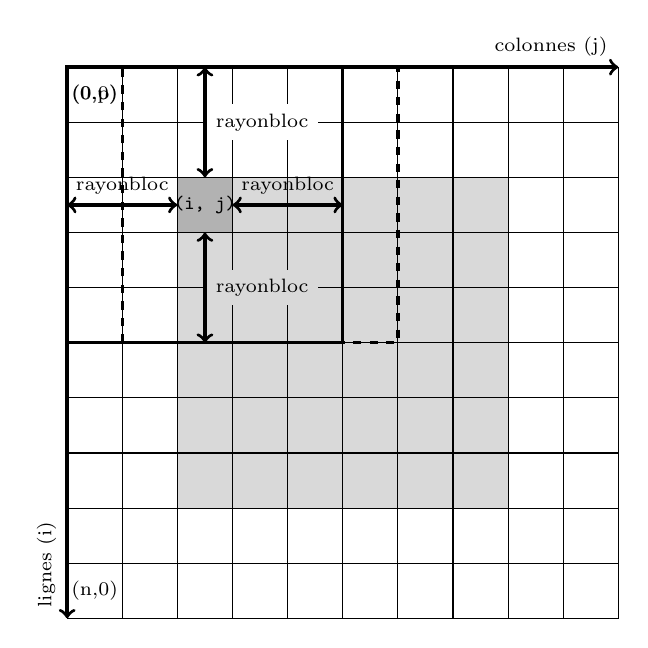
\begin{tikzpicture}[scale=0.7]
 \foreach  \x in {0,...,9}
  {\foreach \y in {0,...,9}
  \draw (\x, \y) rectangle (\x + 1, \y + 1);
  };
   \foreach  \x in {2,...,7}
  {\foreach \y in {2,...,7}
  \filldraw [fill=gray!30,draw=black] (\x, \y) rectangle (\x + 1, \y + 1);
  };
  \draw[very thick] (0,5) rectangle (5,10);
   \draw[very thick, dashed] (1,5) rectangle (6,10);
   \filldraw [fill=gray!60,draw=black] (2,7) rectangle (3,8);
   \draw[<->, very thick] (2.5,8) -- (2.5, 10) node [midway, right,fill=white] {{\scriptsize rayonbloc }};
   \draw[<->, very thick] (2,7.5) -- (0, 7.5) node [midway, above] {{\scriptsize rayonbloc }};
   \draw[<->, very thick] (2.5,7) -- (2.5, 5) node [midway, right,fill=gray!30] {{\scriptsize rayonbloc }};
   \draw[<->, very thick] (3,7.5) -- (5, 7.5) node [midway, above] {{\scriptsize rayonbloc }};
   \draw (2.5, 7.5) node {\scriptsize \texttt{(i, j)}};
   \draw (0.5,9.5) node  {\scriptsize (0,0)};
   \draw (0.5,0.5) node  {\scriptsize (n,0)};
   \draw (0.5,9.5) node  {\scriptsize (0,p)};
   \draw[very thick, ->] (0,10) -- (10,10) node[above left] {\scriptsize colonnes (j)} ;
   \draw[very thick, ->] (0,10) -- (0,0) node[above right, rotate=90] {\scriptsize lignes (i)} ;
    \end{tikzpicture} 
    \end{center} 
\end{minipage}

\bigskip
Si on veut, on peut décider de na pas donner le même poids aux pixels qui entourent le pixel sur lequel on travaille. Autrement dit on peut faire une moyenne coefficientée. Ce calcul est basée sur une matrice qui varie suivant l'effet que l'on veut obtenir. ON dit qu'on fait une convolution.
		
\smallskip
Prenons par exemple la matrice 
$$M = \begin{pmatrix} 1 & 2 & 1 \\ 2 & 4 & 2 \\ 1 & 2 & 1 \end{pmatrix},$$ 
pour la composante rouge, on va remplacer la valeur $r$ d'un pixel par la moyenne coefficientée des valeurs $r$ pour les $8$ pixels alentour et le pixel lui même, affectées des coefficients donnés par la matrice. Et on fera pareil ensuite pour la composante verte et la composante bleue.

\smallskip
Le floutage évoqué précédemment correspond alors à une matrice de taille $3\times 3,\ 5\times 5\ldots$ composée uniquement de 1.


\begin{exoc}{}
\begin{enumerate}
\item Écrire une fonction \verb+moyenne_bloc(pixels, i, j, matrice)+ où \texttt{pixels} est la matrice des pixels de l'image, \texttt{(i,j)} les coordonnées de l'endroit de la matrice où on fait la modification et \texttt{matrice} est la matrice filtre qu'on va utiliser.

\smallskip
\begin{itemize}
\item Il vous faudra distinguer suivant que l'image est en couleur ou en niveau de gris pour opérer sur chacune des composantes.
\item Comme vu un peu plus haut \texttt{numpy} permet des calculs rapides. Par exemple si $M$ et $N$ sont deux matrices de même taille \texttt{M*N} fait le produit terme à terme des deux matrices.
\item Pour faire la somme des éléments d'une matrice vous pourrez utiliser \texttt{np.sum}
\item Si la somme des coefficients de la matrice filtre est non nulle,  on divise le résultat de la convolution par cette somme (moyenne coefficientée) ceci permet de conserver la même luminance globale. Si la somme des coefficients vaut $0$, on divise par $1$.
\end{itemize}
\item Écrire une fonction \verb+applique_filtre(imsource, matrice)+ qui permet d'appliquer un des filtres proposés dans le fichier \texttt{.py} à une image. 

\smallskip
\begin{itemize}
\item On se servira bien évidemment de la fonction de la question précédente.
\item Pour que le bloc ne sorte pas des limites de l'image source, on ne prendra comme centre des blocs que les pixels à une distance \texttt{rayonbloc} des bords (zone grisée sur la figure)
\end{itemize}

\end{enumerate}
\end{exoc}

\Rq Si on effectue la différence entre l'image initiale et l'image floutée on a tendance à accentuer les détails. Par exemple avec la matrice $M$ donnée plus haut on obtient un flou dit gaussien, donc avec la matrice 
$$A=\begin{pmatrix}
0&0&0\\0&20&0\\0&0&0
\end{pmatrix}-M=\begin{pmatrix}
-1&-2&-1\\-2&16&-2\\-1&-2&-1
\end{pmatrix}$$
on obtient une image \og plus nette\fg.

\subsection{Pixellisation}

\begin{exoc}{}

Pour pixelliser une image, l'image est divisée en rectangles de la taille spécifiée (par exemple 10 $\times$ 10 pixels). Chaque rectangle est ensuite rempli avec la couleur moyenne de la zone. Si le côté du bloc n'est pas un diviseur la hauteur et/ou de la largeur de l'image, certaines bandes sur les bord de l'image ne seront pas traitées.

Écrire une fonction \texttt{pixellisation(imsource, taille\_bloc)} qui, étant donnés une image, et le côté d'un bloc, affiche l'image pixellisée.

\textit{On pourra utiliser la fonction} \verb!moyenne_bloc! \textit{donnée plus haut, ou} \texttt{np.mean(matrice)} \textit{qui donne la moyenne des éléments d'une matrice.}

\end{exoc}


\section{D'autres exercices}

\subsection{Seuillage et détection de contour}

\begin{center}
\textit{Nous allons travailler ici sur des images en niveau de gris. Dans vos programme si l'image donnée en entrée n'est pas en niveau de gris on prendra soin de d'abord la transformer en niveau de gris.}
\end{center}

\begin{exoc}{\textit{Seuillage}}

Un filtre de seuillage consiste à mettre à 0 (noir) tous les pixels ayant une valeur inférieure à un certain seuil et à 255 les autres.
Écrire une fonction \texttt{seuil(imsource,s)} qui fait ce qu'on attend d'elle.
\end{exoc}

\begin{exoc}{\textit{Détection de contour}}

Considérons à nouveau dans cet exercice, une image en niveaux de gris. Les bords des objets correspondent à des zones où les valeurs des pixels changent rapidement. C'est le cas par exemple lorsque l'on passe d'un objet clair (avec des valeurs
grandes) à un arrière plan sombre (avec des valeurs petites).
Afin de savoir si un pixel en $({x},{y})$ est le long d'un bord d'un objet, on prend en compte les valeurs des pixels de ces quatre voisins $a,\ b,\ c$ et $d$ (deux horizontalement et deux verticalement).
\begin{center}
  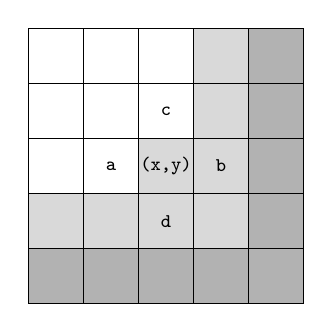
\begin{tikzpicture}[scale=0.7]
  \filldraw [fill=gray!60,draw=black] (0, 0) rectangle (5, 1);
  \filldraw [fill=gray!60,draw=black] (4, 1) rectangle (5, 5);
  \filldraw [fill=gray!30,draw=black] (0, 1) rectangle (4, 2);
  \filldraw [fill=gray!30,draw=black] (3, 1) rectangle (4, 5);
  \filldraw [fill=gray!30,draw=black] (2, 2) rectangle (3, 3);
 \foreach  \x in {0,...,4}
  {\foreach \y in {0,...,4}
  \draw (\x, \y) rectangle (\x + 1, \y + 1);
  };
  \draw (2.5, 2.5) node {\scriptsize \texttt{(x,y)}};
  \draw (1.5, 2.5) node {\scriptsize \texttt{a}};
  \draw (3.5, 2.5) node {\scriptsize \texttt{b}};
  \draw (2.5, 3.5) node {\scriptsize \texttt{c}};
  \draw (2.5, 1.5) node {\scriptsize \texttt{d}};
  \end{tikzpicture} 
\end{center} 

On calcule une valeur $\ell$ suivant la formule : $\ell = \sqrt{(a-b)^2+(c-d)^2}$

\smallskip
On peut remarquer que si $\ell=0$, alors on a $a=b$ et $c = d$ : le pixel n'est pas sur un bord. Au contraire, si $\ell$ est grand, ceci signifie que les pixels voisins ont des valeurs très différentes : le pixel central est donc probablement sur le bord d'un
objet.

\smallskip
On transforme ensuite l'image en affichant du blanc lorsque $\ell$ est faible et du noir lorsque $\ell$ est élevé ; il y a donc une valeur de seuil à déterminer \ldots


Écrire une fonction \texttt{contour(imsource,seuil)} qui fait ce qu'on attend d'elle. On testera cette fonction avec diverses valeurs de seuil.


\textit{On pourra ne pas tenir comptes des pixels au bord de l'image.}
\end{exoc}


\subsection{Transformations géométriques}

\begin{exoc}{\textit{Quart de tour direct}}

On fait subir à l'image initiale une rotation d'un quart de tour direct.
	\begin{enumerate}
	\item Si on a une image de dimension $n\times p$ quelle sera la dimension de l'image obtenue après la transformation ?
	\item Quelles étaient les coordonnées initiales du pixel situé en $(0,0)$ sur l'image finale ?
	\item De manière générale, quelles étaient les coordonnées initiales du pixel situé en $(i,j)$ sur l'image finale ?
	\item Écrire une fonction \verb!quart_tour_direct(imsource)! qui fait ce que son nom indique.
	\end{enumerate}
\end{exoc}

\begin{exoc}{\textit{Réduction}}

Pour réduire une image source  de dimension \texttt{(L, H)}  d'un coefficient \texttt{coef} qui divise L et H, il suffit de créer une image de dimension \texttt{(L // coef, H // coef)} puis pour chaque pixel \texttt{pixel\_res[i, j]} de cette image reçoit la valeur du pixel \texttt{pixels[i * coef, j * coef]} de l'image source.

\begin{enumerate}
\item Compléter le code de la fonction \verb+reduction(imsource, coef)+. 

\item Comment modifier cette fonction pour un agrandissement ? Le résultat sera-t-il satisfaisant ?
\end{enumerate}
\end{exoc}


\subsection{Stéganographie}

\begin{exoc}{\textit{Stéganographie}}

La stéganographie est l'art de la dissimulation : son objet est de faire passer inaperçu un message dans un autre message. Nous allons mettre en œuvre ici un procédé qui permet de cacher des informations dans une image, et plus particulièrement une autre image (mais on peut aussi y dissimuler un texte par exemple).

Voici l'idée directrice : On a vu que chaque pixel d'une image en niveaux de gris peut-être codé par un entier entre 0 et 255. Pour plus de clarté, imaginons, momentanément que les pixels sont codés par des entiers entre 0 et 99. On dispose de deux images de même taille, l'une « anodine » et l'autre « secrète ». On va combiner les pixels des deux images situés à la même place de la façon suivante :
\begin{itemize}
\item Le pixel de l'image anodine est $a_1a_0 = 10a_1+a_0$, celui de l'image secrète est : $s_1s_0 = 10s_1+s_0$
\item On garde la dizaine du pixel de chacune des deux images : $a_1$ et $s_1$
\item On crée un pixel $a_1s_1 = 10a_1 + s_1$ : ainsi à l'affichage, ce pixel est proche du pixel initial : l'image visible est très proche de l'image anodine du départ mais contient tout de même une information sur l'image secrète.
\item Pour révéler, l'image secrète : on prend chaque pixel, on supprime la dizaine, on obtient ainsi l'entier $s_1$, on crée le pixel pour l'image révélée : $10s_1$, qui est donc proche du pixel de l'image secrète.
\end{itemize}
\medskip
Adaptons donc cette méthode dans notre cas où les pixels sont en fait codés avec des entiers 8 bits. Un pixel est codé par un entier $n = \Sum_{i=0}^7 b_i2^i$.
La partie de poids fort à garder (l'équivalent de la dizaine) est $m = \Sum_{i=4}^7 b_i2^i = (n//2^4)$.

On construit le pixel de l'image codée par $p = 2^4 \times m_a + m_s$ ($a$ pour anodin, $s$ pour secret). On décode l'image en extrayant $m_s$ de $p$ en faisant : $m_s=p\%2^4$.
\begin{enumerate}
\item Écrire une fonction qui extrait une image secrète d'une image codée : la tester sur l'image \texttt{mystere.png}.
\item Écrire une fonction qui cache une image secrète dans une image anodine. La tester sur les deux images de même dimension et vérifier avec votre fonction précédente.
\item Faire ce même travail pour des images en couleurs.
\end{enumerate}
\end{exoc}

\Closesolutionfile{Corrige_chp9} 

%\Readsolutionfile{Corrige_chp9}



\faketableofcontents % Pour le bon affichage minitoc
\end{document}


%%%%%%%%%%%%%%%%%%%%%%%%%%%%%%%%%%%%%%%%%%%%%%%%%%%%%%%%%%%%%%%%%%%%%%%%%%%%%%%%%%
%%%%%%%%%%%%%% D'autres exercices
%%%%%%%%%%%%%%%%%%%%%%%%%%%%%%%%%%%%%%%%%%%%%%%%%%%%%%%%%%%%%%%%%%%%%%%%%%%%%%%%%%

\begin{exoc}{\textit{Amélioration des contours}\hfill \textit{Ne pas traiter cet exercice dans un premier temps.}}

Le but est d'améliorer les images binaires (noir et blanc) obtenues aux exercices précédents : on cherche à \og fermer \fg{} les contours de l'image. Pour cela nous allons procéder en trois étapes.

\medskip

Dans un premier temps nous allons \og nettoyer \fg{} l'image en enlevant tous les pixels noirs isolés.
\begin{center}
Si le pixel en $(x,y)$ est noir et que tous ces voisins sont blancs on le coloris en blanc.
\end{center}

Ensuite on va dilater les contours. Pour cela on crée une nouvelle image avec la méthode suivante :
\begin{center}
le pixel en $(x,y)$ est colorié en noir si au moins un de ses voisins est noir, sinon on le colorie en blanc.
\end{center}

Enfin la dernière étape consiste à \og éroder\fg{}. L'érosion est l'opération duale de la dilatation. On crée encore une nouvelle image à partir de l'image précédente de la manière suivante :
\begin{center}
le pixel en $(x,y)$ est colorié en noir si tous ses voisins sont noirs, sinon on le colorie en blanc.
\end{center}
En appliquant ainsi un opérateur de dilatation suivi d'un opérateur d'érosion à l'image binaire, on dit que l'on fait une fermeture de l'image binaire. Cette technique est utilisée pour améliorer les images de documents scannés.

\begin{enumerate}
\item Écrire une fonction \texttt{nettoyage(imsource)} qui fait ce qu'on attend d'elle.
\item Écrire une fonction \texttt{dilatation(imsource)} qui fait ce qu'on attend d'elle.
\item Écrire une fonction \texttt{erosion(imsource)} qui fait ce qu'on attend d'elle.
\item Écrire une fonction \texttt{amelioration(imsource)} qui fait ce qu'on attend d'elle.
\end{enumerate}
\end{exoc}


\begin{exoc}{\textit{Détection de contour}\hfill \textit{Ne pas traiter cet exercice dans un premier temps.}}

Un pixel est sur le contour d'un objet s'il y a une forte variation de couleurs autour de ce pixel. Pour le pixel en $(x,y)$, on se propose donc 
\begin{itemize}
\item de comparer la variation de la composante rouge entre les deux voisins du dessus et du dessous ce qu'on note ainsi (pour comprendre, pas en python) : $\left|r(x,y+1)-r(x,y-1)\right|$, et de faire de même pour les autres composantes.
\item puis de comparer la variation de la composante rouge entre les deux voisins de gauche et de droite : $\left|r(x-1,y)-r(x+1,y)\right|$, et de faire de même pour les autres composantes.
\end{itemize}
On fait la somme de ces 6 valeurs (2 pour chaque composante), et on obtient une valeur de la variation de couleur autour de ce pixel. En seuillant cette variation, on détermine si le pixel  en $(x,y)$ est sur le contour d'un objet,  et donc s'il doit être blanc ou noir.

Écrire une fonction \texttt{contour(imsource,seuil)} qui fait ce qu'on attend d'elle.

\textit{On pourra ne pas tenir comptes des pixels au bord de l'image.}
\end{exoc}